% ONE-NAS paper — working draft assembling all completed results.
% Venue styling (IAAI/AAAI) to be applied later; article class for now.
% Sources: PAPER_MAP.md; tables from icaif_window_tables.tex,
% m1_ensemble_table.tex, hp_reporting.tex; figure net_curves.pdf.
\documentclass[11pt]{article}
\usepackage[margin=1in]{geometry}
\usepackage{booktabs}
\usepackage{threeparttable}
\usepackage{amsmath}
\usepackage{graphicx}
\newcommand{\se}[1]{{\scriptsize$\pm$#1}}
\title{Online Neuroevolution as an Ensemble Generator:\\
Island-Champion Aggregation for Cost-Aware Stock Return Prediction}
\author{Anonymous Author(s)}
\date{Working draft --- 2026-08-29}
\begin{document}
\maketitle

\begin{abstract}
Online neuroevolutionary architecture search (ONE-NAS) maintains a
population of small recurrent networks that evolves continuously as a data
stream arrives. Its published prediction rule --- forecast with the single
best genome --- presumes that the search can identify its best network. On
equity return panels it cannot: validation fitness is nearly uncorrelated
with realized economic quality, and the single champion underperforms a
plain online LSTM. We show that the population is nevertheless valuable ---
as an \emph{ensemble generator}. Aggregating each island's champion by
rank-mean turns the same completed runs into the strongest system in a
cost-aware prequential evaluation on CRSP mid-cap panels: within-run, the
ensemble beats the single champion by $+23.0$ net points over 2022--2024
(paired $t{=}18.2$ over ten seeds), a gain that widens with island count,
replicates on a disjoint 2016--2019 span, is positive in all fifteen
hyperparameter configurations we trained, and matches the ensemble-averaging
prediction from measured member diversity to within 4\%. The resulting
system exceeds online LSTM/GRU and periodic-retraining baselines under
identical books and costs, is the only arm with significant factor-model
alpha ($+7.9\%$/yr, Newey--West $t{=}2.14$), and its always-online population
appreciates: a cold start forfeits roughly half the profit. The networks
are tiny (tens of weights per member), making the entire system --- search
included --- deployable on commodity single-board hardware.
\end{abstract}

\section{Introduction}
Time-series forecasting models are typically compared on pointwise error,
yet a lower forecast error need not imply a better trading decision. The
prior work in this line compared offline-evolved recurrent networks (EXAMM)
against modern forecasters under a daily long--short protocol and found the
evolved networks strongest. This paper studies the \emph{online} variant,
ONE-NAS, under a continuously evolving population, and makes four
contributions:
\begin{enumerate}
\item \textbf{A prediction rule for online NAS}: rank-mean aggregation of
island champions, replacing the published single-genome rule.
\item \textbf{A cost-aware prequential protocol} on CRSP mid-cap panels:
pooled cross-sectional training, netted half-spread costs, paired
seed-level statistics, and a pre-registered configuration ledger.
\item \textbf{A mechanism study} showing \emph{why} aggregation is the
right rule: fitness is uninformative for selection on this domain, so the
population's value is only accessible by averaging --- and the gain matches
diversity theory quantitatively.
\item \textbf{An online-continuity result}: the deployed population is an
appreciating asset; cold-starting forfeits about half the profit.
\end{enumerate}

\section{Method}
ONE-NAS extends EXAMM neuroevolution to streaming data: islands of small
recurrent genomes (evolvable node types: simple, UGRNN, MGU, GRU,
$\Delta$-RNN, LSTM; deep recurrent connections with time-skips) train
online as each new window of the stream arrives, with island extinction
and repopulation maintaining structural diversity. The published system
predicts with the single global-best genome. We instead form, at every
generation, the \textbf{rank-mean ensemble of the island champions}: each
island's best genome produces a cross-sectional prediction; predictions
are rank-transformed per day and averaged. Islands evolve in isolation and
exchange genetic material only through rare inter-island crossover, so
champions are structurally diverse; their measured pairwise prediction
correlation is $\rho \approx 0.17$--$0.22$, the diversity that aggregation
harvests.

\section{Data and evaluation protocol}
\textbf{Panels.} Four 50-stock mid-cap panels ($V1$--$V4$) drawn from CRSP,
identical to the prior paper's validation portfolios. Inputs are seven
per-stock features (return, cross-sectional rank input, bid--ask spread,
Amihud illiquidity, 21-day reversal, turnover ratio, 21-day volatility);
the target is the next-day cross-sectional rank-normal return. Feature
normalization is frozen at the 2019 burn-in boundary; realized returns for
all economics are CRSP total returns (split- and dividend-adjusted).

\textbf{Clock.} Prequential: sliding windows of length 40 advance 5 trading
days per generation; no prediction uses information after its date. The
population evolves from 2020-01 onward; headline evaluation uses
2022--2024, the prior paper's test years, with the full 2020--2024 span in
the appendix.

\textbf{Book.} Predictions trade through overlapping-sleeve top-10/bottom-10
long--short portfolios (Jegadeesh--Titman construction, 10-day holding,
1/10 of capital per day), charged the half quoted spread on netted traded
notional. The book reads only the cross-sectional \emph{order} of
predictions and is invariant to monotone rescaling.

\textbf{Statistics.} The comparison unit is one training run. Ten seeds
(42--51) per configuration; metrics are averaged over panels within seed
and tested by paired $t$ across seeds; daily quantities use HAC standard
errors. The system configuration was frozen in a pre-registered ledger
before confirmatory scoring; hyperparameters were selected on 2016--2019
data only (Section~\ref{sec:hps}).

\section{Headline results}
Table~\ref{tab:window} compares ONE-NAS on the evaluation window against
the prior paper's published EXAMM and buy-and-hold rows, under three
portfolio constructions. Figure~\ref{fig:curves} shows the cumulative net
paths. ONE-NAS is profitable in every trade year including the 2022
drawdown, and is the only arm whose factor-model alpha is significant:
regressing pooled daily book returns on the Fama--French three factors
plus momentum (Newey--West lag 10) gives $+7.9\%$/yr ($t{=}2.14$, market
beta $0.12$) for the 40-island system, against $t \le 1.8$ for every
baseline and a beta-0.97 buy-and-hold control at $t{=}0.4$.

\begin{table}[t]
\centering
\begin{threeparttable}
\caption{Net return (\%) by trade year, mean over $V1$--$V4$. ONE-NAS books
are restarted at each window boundary; the 2022--24 column is one book run
over the three-year window.}
\label{tab:window}
\begin{tabular}{lrrrr}
\toprule
 & 2022 & 2023 & 2024 & 2022--24 \\
\midrule
ONE-NAS (40 isl., sleeves book)              & $+6.1$\se{0.8}  & $+12.4$\se{0.7} & $+6.4$\se{0.5}  & $+27.5$\se{1.1} \\
ONE-NAS (40 isl., banded book)\tnote{a}      & $+12.5$\se{1.2} & $+14.6$\se{1.3} & $+3.4$\se{0.9}  & $+33.9$\se{1.8} \\
ONE-NAS (40 isl., Algorithm 1 book)\tnote{b} & $+1.3$\se{1.6}  & $+12.8$\se{1.0} & $+10.8$\se{1.2} & $+25.0$\se{1.8} \\
\midrule
ONE-NAS single champion (8 isl., sleeves)\tnote{c} & $+3.1$\se{1.8} & $+1.7$\se{1.3} & $+2.7$\se{1.1} & $+8.5$ \\
Online LSTM (sleeves book)                   & $+1.2$\se{1.3}  & $+4.5$\se{1.2}  & $+3.8$\se{0.7}  & $+11.3$\se{1.8} \\
\midrule
EXAMM (prior paper)                          & $+15.5$         & $+9.1$          & $+8.5$          & $+33.1$\tnote{d} \\
Buy \& hold (prior paper)                    & $-10.1$         & $+11.2$         & $+6.8$          & $+7.9$\tnote{d} \\
\bottomrule
\end{tabular}
\begin{tablenotes}\footnotesize
\item[a] Buy/hold-spread rule: enter at rank $\le$10 per side, exit when
rank decays past 35 (Novy-Marx \& Velikov 2016). Winner of a seven-book
sensitivity sweep on the development span; reported as sensitivity, not an
adopted headline.
\item[b] The prior paper's conditional long--short book applied verbatim.
On rank-normal predictions its entry gate fires every day (average holding
1 day vs.\ EXAMM's $\approx$5), an $\approx$8\%/yr cost drag; conservative
for ONE-NAS.
\item[c] The published ONE-NAS prediction rule; seeds 42--44 ($n{=}3$).
\item[d] Prior-paper rows are its published Table 7 yearly cells from its
own trading stack; their 2022--24 column is the sum of yearly cells.
\end{tablenotes}
\end{threeparttable}
\end{table}

\begin{figure}[t]
\centering
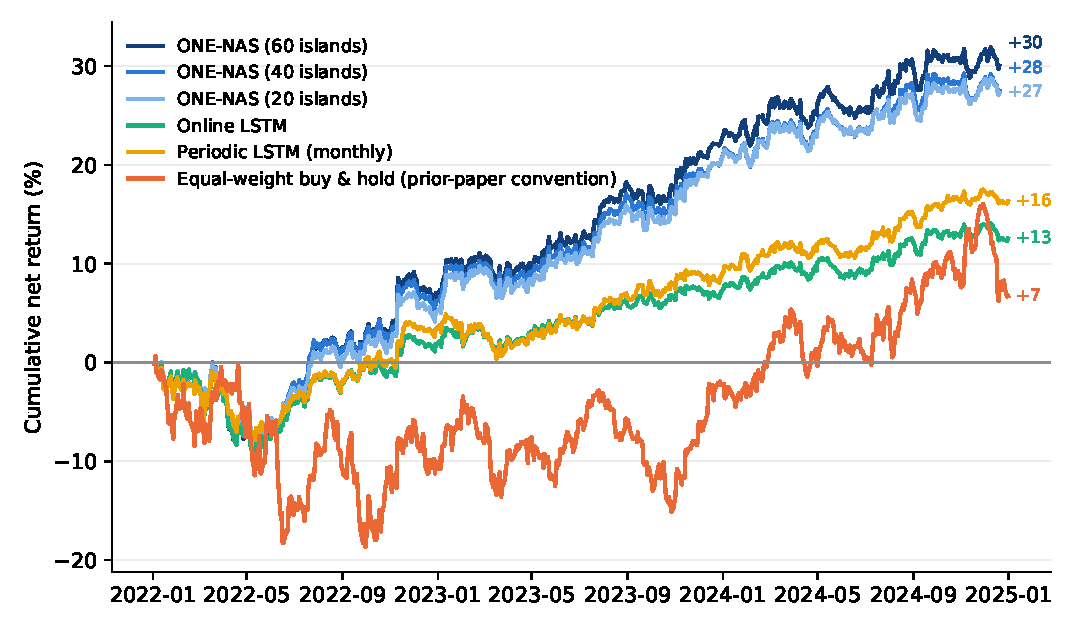
\includegraphics[width=\linewidth]{net_curves.pdf}
\caption{Cumulative net return, 2022--2024 (books restarted at the window
start; endpoints match Table~\ref{tab:window}). Buy-and-hold follows the
prior paper's benchmark convention.}
\label{fig:curves}
\end{figure}

\section{Why it works: aggregation, not selection}
\label{sec:mech}
\textbf{The fitness signal cannot select.} The rank correlation between a
genome's validation MSE and its realized next-week economic quality is
$+0.02$; given a fixed pool ten times the usual size, selecting the argmax
buys $+0.022$ daily rank IC while simply averaging the pool buys $+0.143$;
a random pick beats the argmax. The identical harness passes its positive
control on NAS-Bench-201, so the limitation is the domain's, not the
tooling's: at this signal-to-noise, per-genome quality is unselectable.

\textbf{Within-run test.} Table~\ref{tab:m1} extracts both prediction
rules from the same completed runs. The ensemble wins at every fleet,
window, and metric ($t$ from 4.5 to 18.2); the single champion
\emph{degrades} as islands widen (more lottery tickets for an
uninformative selector) while the ensemble improves --- the winner's curse
and its cure in one table. The contrast replicates on 2016--2019, a span
that played no role in adopting the ensemble rule.

\begin{table}[t]
\centering
\begin{threeparttable}
\caption{Prediction rule, within-run paired: single global-best genome
vs.\ island-champion rank-mean ensemble from the same runs. Net \% /
Sharpe; $\Delta$ = ensemble $-$ single, paired $t$ over seeds.}
\label{tab:m1}
\begin{tabular}{llrrrr}
\toprule
Fleet & Window & Single & Ensemble & $\Delta$net ($t$) & $\Delta$Sharpe ($t$) \\
\midrule
40 isl.\ ($n{=}10$) & 2022--24 & $+4.5$ / $0.21$  & $+27.5$ / $0.87$ & $+23.0$ $(18.2)$ & $+0.66$ $(14.7)$ \\
40 isl.\ ($n{=}10$) & 2020--24 & $+2.7$ / $0.08$  & $+45.6$ / $0.68$ & $+42.9$ $(14.6)$ & $+0.60$ $(13.4)$ \\
8 isl.\ ($n{=}10$)  & 2022--24 & $+8.3$ / $0.33$  & $+20.5$ / $0.70$ & $+12.2$ $(6.7)$  & $+0.37$ $(5.8)$ \\
8 isl.\ ($n{=}10$)  & 2020--24 & $+12.0$ / $0.21$ & $+32.1$ / $0.52$ & $+20.1$ $(5.5)$  & $+0.30$ $(5.3)$ \\
\midrule
8 isl.\ ($n{=}5$)\tnote{a}  & 2016--19 & $+16.3$ / $0.56$ & $+26.0$ / $0.92$ & $+9.7$ $(5.2)$   & $+0.36$ $(4.5)$ \\
40 isl.\ ($n{=}5$)\tnote{a} & 2016--19 & $+8.9$ / $0.30$  & $+36.7$ / $1.22$ & $+27.8$ $(7.5)$  & $+0.92$ $(6.6)$ \\
\bottomrule
\end{tabular}
\begin{tablenotes}\footnotesize
\item[a] Robustness replication on the 2016--2019 tuning-span fleets.
\end{tablenotes}
\end{threeparttable}
\end{table}

\textbf{The gain is quantitatively explained by diversity.} With measured
member rank IC $m$ and pairwise prediction correlation $\rho$, the
equicorrelated averaging prediction $m\sqrt{N/(1+(N-1)\rho)}$ matches the
measured ensemble IC within 4\% in all four fleets (e.g.\ 40 islands:
predicted $+0.0132$, measured $+0.0128$ at $\rho{=}0.172$). Wider
populations are more diverse ($\rho$ 0.216 at 8 islands vs.\ 0.172 at 40),
which is where width's ensemble gain originates; width otherwise buys
reliability (seed dispersion of Sharpe falls from 0.171 to 0.078), not
mean IC.

\textbf{The gain is configuration-invariant.} Re-scoring both prediction
rules inside all fifteen hyperparameter configurations we ever trained
(Section~\ref{sec:hps}) gives a positive within-run ensembling net gain in
15/15 cells (mean $+8.2$, up to $+20.6$, $t{=}6.0$); it shrinks toward zero
only in the two IC-selection cells whose populations are degenerate ---
aggregation harvests diversity from healthy populations.

\textbf{Boundary.} Random-architecture online ensembles match evolved
champions at the registered book ($t{=}0.41$): on this domain, evolution's
contribution beyond generating diverse small architectures is not
detectable, and aggregation doubles Sharpe across all member-generation
mechanisms. We state this as a scope condition on the method's value.

\section{Online continuity}
Deploying the frozen configuration cold at 2022-01 earns $+12.3$ pooled
net over 2022--2024 versus $+26.5$ for the same window inside runs that
had been evolving online since 2020 --- the always-online population is an
appreciating asset, and this is what online search buys over periodic
retraining (a generation-count confound is disclosed in the artifact).

\section{Hyperparameters}
\label{sec:hps}
ONE-NAS hyperparameters were selected by single-factor search scored on
2016--2019 validation data, disjoint from the 2020--2024 evaluation span;
the search covered island count (8--40), elite and generated population
sizes (including the originally published 5/10), repopulation frequency
(25--100), training-subsequence count (600--2000), sequence length (15,
40), backpropagation epochs (10, 20), replay-priority parameters, rounds
per generation, selection metric (validation MSE vs.\ rank-IC variants),
and target horizon (1- and 5-day cross-sectional). The selected settings
are given in Table~\ref{tab:hps}; complete per-configuration results are
available in the project repository. Two findings are noteworthy:
selecting genomes by validation rank-IC \emph{harms} economics
($-0.55$ to $-0.90$ Sharpe), consistent with
Section~\ref{sec:mech}'s unselectability result; and no variant beat the
selected configuration on the tuning objective.

\begin{table}[t]
\centering
\caption{ONE-NAS hyperparameter settings.}
\label{tab:hps}
\begin{tabular}{ll}
\toprule
Hyperparameter & Value \\
\midrule
Islands & 40 (headline); 8 (registered primary) \\
Elite population per island & 8 \\
Generated genomes per island per generation & 5 \\
Repopulation frequency & every 50 generations \\
Selection metric & validation MSE \\
Prediction rule & rank-mean ensemble of island champions \\
Target & 1-day cross-sectional rank-normal return \\
Sequence length / window step / validation sets & 40 / 5 / 5 \\
Training subsequences per genome & 2000 \\
Backpropagation epochs per genome & 10 \\
Replay (PER) $\alpha$, $\lambda$, $\epsilon$ & 0.6, 0.007, $10^{-8}$ \\
Rounds per generation & 1 \\
Node-type library & simple, UGRNN, MGU, GRU, $\Delta$-RNN, LSTM \\
Mutation / intra- / inter-island crossover & 0.7 / 0.2 / 0.1 (EXAMM defaults) \\
Warm-up generations & 50 \\
\bottomrule
\end{tabular}
\end{table}

\section{Deployment}
Each ensemble member averages tens of weights; even the 40-champion
ensemble totals $\approx$2{,}600 parameters, orders of magnitude below the
transformer baselines of the prior study. The search itself is CPU-only
with a weekly decision clock, giving large headroom for on-device
operation; on-device measurements (ensemble inference and one weekly
evolution generation on single-board hardware) and live-pilot status are
reported in the final version. [D1/D2 measurements and pilot paragraph to
be inserted.]

\section{Limitations}
The evaluation window (2022--2024) is inherited from the prior paper's
protocol and lies within this project's development span; full-span
results and the configuration ledger are provided for transparency. The
universe carries survivorship bias from drawing current constituents
backward. Results cover one market, one frequency, and mid-cap panels;
the random-architecture boundary result limits claims about evolutionary
search per se, as opposed to the online-population-plus-aggregation
system. Prior-paper comparison rows follow that paper's published
benchmark convention, noted where used.

\end{document}
